\chapter{二分圖匹配}

\> 匹配(matching)是圖論裡一個重要的問題,而相關的演算法可以推廣到許多不同的題目。

\section{匹配問題介紹}

\subsection{名詞解釋}

\begin{enumerate}
	\item 匹配 (Matching): 一個無向圖$G = (V, E)$的邊集$M$,使得$M \subseteq E$ 且$M$裡面任兩條邊都沒有共用點時,$M$稱為圖$G$的匹配。
	\item 匹配邊 (Matched Edge): 被選在目前匹配裡的邊。
	\item 匹配點 (Matched Vertex): 某個匹配邊的端點。
	\item 極大匹配 (Maximal Matching): 一個匹配$M$不存在匹配$M'$使得$M \subset M'$時稱為極大匹配。
	\item 最大匹配 (Maximum Matching): 所有匹配中邊數最多者。沒特別註明時,以下用$|M|$表示最大匹配的大小。
	\item 完美匹配 (Perfect Matching): 所有點都是匹配點的匹配。
	\item 點(邊)覆蓋 (Vertex/Edge cover): 圖上的一個點(邊)集使得所有邊(點)都和該集合的點(邊)相鄰。 
	\item (點)獨立集 (Independent Set):圖上的一個點集\(I\)使得\(I\)內任兩個點不相鄰。
\end{enumerate}

\pagebreak
我們可以用下面一張圖舉例:

\begin{center}
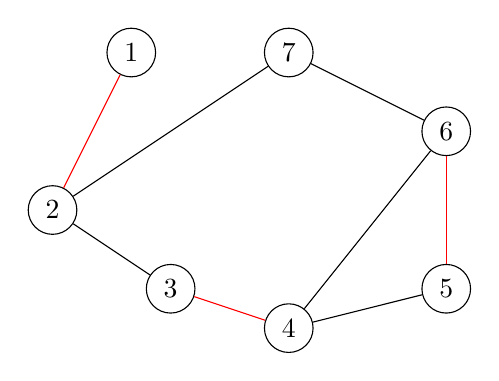
\begin{tikzpicture}[every node/.style={circle,draw=black}]
	\node (1) at (0, 5) {1};
	\node (2) at (-1, 3) {2};
	\node (3) at (0.5, 2) {3};
	\node (4) at (2, 1.5) {4};
	\node (5) at (4, 2) {5};
	\node (6) at (4, 4) {6};
	\node (7) at (2, 5) {7};

	\draw[red] (1) -- (2);
	\draw (2) -- (3);
	\draw[red] (3) -- (4);
	\draw (4) -- (5);
	\draw[red] (5) -- (6);
	\draw (6) -- (7);
	\draw (2) -- (7);
	\draw (4) -- (6);
\end{tikzpicture}
\end{center}

其中,紅色的邊代表一組匹配。此匹配為其中一個極大匹配,也是最大匹配。若選擇$(2, 7), (6, 4)$兩條邊,則該匹配為極大匹配,但不是最大匹配。

\subsection{匹配問題與其分類}
匹配問題通常分為四種,分別為:最大匹配 (maximum matching) 、最小邊覆蓋 (minimum edge cover) 、最小點覆蓋 (minimum vertex cover) 、和最大獨立集 (maximum independent set)。
\par 在一般圖最大匹配與最小邊覆蓋屬於P問題,最小點覆蓋與最大獨立集則為NP-Hard。這四個問題本身也存在著這個對應關係,我們可以透過以下引理來了解。
\lemma{匹配問題的對應}{
在一張連通圖$G = {V, E}$中,
\[|\textrm{最大匹配}| + |\textrm{最小邊覆蓋}| = |\textrm{最小點覆蓋}| + |\textrm{最大獨立集}| = |V|\]
}
這裡證明最大匹配和最小邊覆蓋大小總和是$|V|$。在最小邊覆蓋問題裡面,我們要用最少的邊數覆蓋到所有的點,所以每一條邊一定會覆蓋一個沒被其他邊覆蓋的點(否則那條邊刪掉也沒差),因此可以看成是每一條邊貢獻$1$到$2$個點,希望能最大化貢獻$2$個點的邊數。那麼假設最大匹配大小為$M$,有$|V| - 2M$個點已經被覆蓋了,剩下的每次只能用一條邊覆蓋掉一個點,所以邊覆蓋大小為$M + |V| - 2M = |V| - M$。最小點覆蓋的部份留給讀者證明。
\par 另外,在二分圖上,最大匹配的大小恰等於最小點覆蓋的大小(詳細證明在之後章節),而且二分圖的最大匹配好寫很多,學會的話會是十分好用的演算法。

\section{二分圖匹配演算法}

我們先考慮一個最簡單的想法:如果能加一條邊到目前的匹配裡就直接比他加進去。這樣顯然會是錯的,以下列的圖為例:
\begin{center}
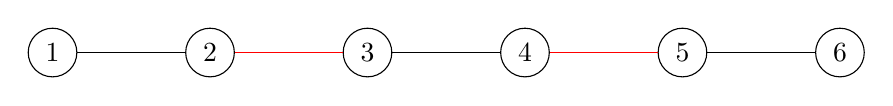
\begin{tikzpicture}[every node/.style={circle,draw=black}]
	\node (1) at (-4, 0) {1};
	\node (2) at (-2, 0) {2};
	\node (3) at (0, 0) {3};
	\node (4) at (2, 0) {4};
	\node (5) at (4, 0) {5};
	\node (6) at (6, 0) {6};

	\draw (1) -- (2);
	\draw[red] (2) -- (3);
	\draw (3) -- (4);
	\draw[red] (4) -- (5);
	\draw (5) -- (6);
\end{tikzpicture}
\end{center}
\par 顯然的,全部選黑色的邊會比選紅色的邊還好,那這是為什麼呢?原本選紅色的時候,$2, 3, 4, 5$是匹配點,改成黑色邊的時候他們都還是匹配點,而新增了$1, 6$兩個匹配點。也就是說,從$1$這個未匹配點開始,沿著黑色邊和紅色邊交替的路徑走,走到另一個未匹配點時,就可以把途中的匹配邊和未匹配邊交換,得到一個更大的匹配!有了這樣的直覺後,就可以看下面的一些定義。
\definition{交替路徑與增廣路徑}{
\begin{itemize}
    \item 交替路徑 (alternating path) :圖上由匹配邊和未匹配邊交替形成的路徑。
    \item 增廣路徑 (augmenting path) :兩端點皆為未匹配點的交替路徑。
    \item 擴增:將增廣路徑上的未匹配邊和匹配邊交換。
\end{itemize}
}
我們前面在描述的就是增廣路徑,而現在我們知道了有增廣路徑的匹配還可以變大,那是不是沒有增廣路徑的匹配一定是最大的呢?
\theorem{Berge's Lemma}{
一個匹配是最大匹配若且唯若不存在增廣路徑。
}
\par 證明:假設$M, M'$是圖$G$的匹配,且$|M| < |M'|$,我們想要證明$M$上一定存在增廣路徑。考慮$M$跟$M'$的對稱差$G' = (M \backslash M') \cup (M' \backslash M)$,也就是圖$G$中,只存在$M$或$M'$其中一個的邊。可以知道$G'$的每個點度數$\leq 2$,且如果度數是$2$的話一定是連到一條$M$和一條$M'$的邊。因此$G'$會由孤點、交錯偶環和交錯路徑構成。因為$|M'| > |M|$,多的那些邊一定是出現在交錯路徑上,也就代表$M$上面的增廣路徑存在。
\par 有了這個定理後,我們就得到一個演算法:維護當前的匹配\(M\),持續擴增直到沒有增廣路徑為止。那要怎麼找到擴增路徑呢?
\par 因為我們討論的是二分圖,所以一條擴增路徑的起終點一定在二分圖的兩邊。因此,我們可以枚舉其中一側的所有點,從該點開始DFS,找到增廣路徑的話就擴增。用下面的圖片可能會更好理解:
\begin{center}
\includegraphics[scale=0.3]{images/Matching/AlternatingTree.png}
\end{center}
這是從最左邊的(未匹配)點開始,只走交替路徑出來的DFS樹,又稱作交替路徑樹。當我遇到一個增廣路徑時就能直接換邊然後回傳,每次最多增加一條匹配邊。複雜度是$V$次DFS的時間,也就是$O(VE)$。
\begin{C++}
int n, m; //1-base
int mx[maxn], my[maxn]; //兩邊匹配對應到的點
bool adj[maxn][maxn], vis[maxn];
bool dfs(int n) {
	if (vis[n]) return false;
	vis[n] = 1;
	for (int v = 1;v <= n;v++) {
		if (!adj[n][v]) continue;
		if (!my[v] || (my[v] && dfs(my[v]))) { //有增廣路徑的話
			mx[n] = v, my[v] = n;
			return true;
		}
	}
	return false;
}
int main() {
	// 輸入圖
	int cnt = 0;
	for (int i = 1;i <= n;i++) {
		for (int j = 1;j <= n;j++) vis[j] = 0; //記得重設 visited
		if (dfs(i)) {
			cnt++;
		}
	}
    cout << cnt << endl;
}
\end{C++}
\subsection{一些實作細節}
\par 如果我們在開始找增廣路徑之前,先 greedy 的求出一個極大匹配,那麼執行速度會快上許多。這是因為任何極大匹配的大小至少是最大匹配大小的一半。而實際上雖然$O(VE)$的複雜度看起來很大,但是他帶的常數極小,通常$V$到$1000$,甚至到$2000$都可能可以使用這個演算法。

\par 其實二分圖匹配還可以做到$O(\sqrt{V} E)$,有興趣的人可以查 \href{https://en.wikipedia.org/wiki/Hopcroft-Karp_algorithm}{Hopcroft-Karp Algorithm},而另外用 Dinic 實作最大流也可以得到$O(\sqrt{V} E)$的時間。

\section{二分圖最小點覆蓋}
前面有提到,最小點覆蓋在一般圖上是NP-Hard問題,但是在二分圖上,大小卻剛好跟最大匹配一樣。以下會介紹他的證明,以及構造解的方法。
\theorem{König's Theorem}{
在二分圖上,最大匹配的大小和最小點覆蓋大小相同。
}
這個定理可以用線性規劃的對偶或是數學歸納法等方法證明,不過最直接且常見的證明方式是用構造法。以下會試著用一個比較直觀的方法說明此構造的動機是什麼。
以下圖的二分圖為例:
\begin{center}
    \includegraphics[width=4cm]{images/Matching/VertexCover1.png}
\end{center}
令二分圖的兩邊的點集合分別為$L, R$。
\par 我們想要選最少的點使得所有邊的其中一個端點都是我們選的點。首先可以發現這個大小必須$\geq |M|$,也就是最大匹配的大小,因為最大匹配的邊都不共點,一個點只能覆蓋到最多一條匹配邊。因此,如果要點覆蓋大小為$|M|$的話,選的點一定是匹配點。接著考慮一個在$L$的未匹配點$u$,他連接到的點$v_1, \dots, v_k$都必須選起來,而\textbf{這些點一定是匹配點,否則會有增廣路徑},那麼他們匹配到的點$u'_1, \dots, u'_k$連出去的邊也就會空出來,變成跟未匹配點$u$一樣的情況。
\par 持續這樣選之後,考慮這個過程中未經過的點(白色)左邊的所有點都是匹配點,因此把他們選起來就能覆蓋剩下的所有邊,最後的點覆蓋為下圖中的綠色點。這個過程中所有匹配邊都只有其中一個匹配點被覆蓋,故點覆蓋大小與最大匹配大小相同。
\begin{center}
    \includegraphics[width=4cm]{images/Matching/VertexCover2.png}
\end{center}
上面是比較白話的理解方式,而接下來用一些符號來做更嚴謹的證明。
\par 令$U$為$L$中的未匹配點(深藍色),$T$是從$U$走交替路徑經過的點,其中左邊稱為$T_L$,右邊為$T_R$。那麼一個最小點覆蓋的可行解為$(L \backslash T_L) \cup T_R$。
\par 首先證明這真的是一個點覆蓋,也就是說不存在邊$(x, y)$使得$x \in T_L,y \in (R \backslash T_R)$。假設$x \in T_L$,若此邊是匹配邊,那$U$是從這條邊走到$x$的,$y \in T_R$。否則如果是未匹配邊且$y \in (R \backslash T_R)$,從$U 	\rightsquigarrow x \rightarrow y$就是增廣路徑,與最大匹配的假設矛盾。
\par 再者說明點覆蓋大小與最大匹配相同。每個$L \backslash T_L$的點和$T_R$的點都是匹配點,而且$T_R$匹配到的點會在$T_L$裡,故一條匹配邊恰有一點被選到,證明完成。
\par 講了這麼多,構造最小點覆蓋的實作方式應該也很明顯了,只要從左邊的未匹配點一個個DFS,標記出$L \backslash T_L$和$T_R$的點即可。
\begin{C++}
int n, m;
int mx[maxn], my[maxn];
bool adj[maxn][maxn], vis[maxn], cx[maxn], cy[maxn]; 
void dfs2(int n) {
	if (vis[n]) return;
	vis[n] = 1;
	cx[n] = 0;
	for (int v = 1;v <= m;v++) {
		if (!adj[n][v]) continue;
		cy[v] = 1;
		if (my[v]) {
			dfs2(my[v]);
		}
	}
}
int main() {
    //先找最大匹配
    for (int i = 1;i <= n;i++) {
    	cx[i] = 1, vis[i] = 0;
    }
	for (int i:u) dfs2(i);
	//cx[i] == 1 代表選左邊點 i, cy[i] == 1 代表選右邊點 i
}
\end{C++}

到了這邊,IOI課綱內匹配的知識已經介紹完畢(其實筆者不知道最小點覆蓋可不可以考)。那麼接下來就是練習一些相關的題目了。
\problem{\href{https://tioj.ck.tp.edu.tw/problems/1069}{TIOJ 1069}}{
在二維平面上有$n$個緊急事件,第$i$個位於$(x_i, y_i)$,並會在時間$t_i$發生。你需要指派警察去處理事件。一個警察一開始可以出現在任意位置,之後每單位時間能朝上下左右移動一格(或不動)。警察必須要在事件發生時位於事件的位置,問最少需要幾個警察才能處理所有事件。
}
\par 首先,我們先把每個事件視為圖上的一個點,如果完成$u$事件之後趕得上$v$事件,就連一條$(u, v)$的有向邊。那麼問題可以看成:在一張有向無環圖上用最少的路徑數量覆蓋所有點。
\par 這看起來非常的難做,畢竟沒有一個直接的greedy選法。一個可能的想法是,假設從$n$個路徑(每個路徑只是一個點)開始,只要有兩個路徑$x, y$,使得$x$的結尾走得到$y$的開頭,就可以合併成一條路徑。這樣的話,要做的事情就是最大化合併的次數。
\par 假設我們建一張二分圖,兩邊各$n$個點,原本的圖上如果$u$走得到$v$就把左邊點$L_u$連到右邊$R_v$。那麼合併路徑$x, y$就可以想成選圖上的邊$(L_x, R_y)$。因為一個路徑的結尾只能跟最多一個路徑的開頭合併,所以在二分圖上選的邊必須是匹配。而對於任何一個匹配,都存在一組路徑可以對應到該匹配,因此本題的答案為$n - |M|$。
\par 註:本題在建有向圖時,$(u, v)$有連邊和$u$走得到$v$是等價的,但是在推廣的問題(DAG最小路徑覆蓋)裡轉換到二分圖時,要看的是$u$走得到$v$的條件。
\section{習題 Part 1}
此處習題為二分圖最大匹配和最小點覆蓋的習題,這類問題的重點就是找到建圖的方式,以及匹配或點覆蓋代表的意義。
\problem{\href{https://csacademy.com/contest/archive/task/flipping-matrix/}{Flipping Matrix}}{
給一個 $n \times n, n \leq 10^3$的01矩陣。每次操作可交換任兩行,或任兩列。請輸出一組操作使得主對角線上面的格子都是$1$,最多做 $n^2$ 次操作,若無解輸出$-1$。
}
\problem{\href{https://tioj.ck.tp.edu.tw/problems/1253}{TIOJ 1253 砲打皮皮}}{
在一個$n\times n$的棋盤上面有一些怪物,每次可以選擇一直行或一橫列消除所有的怪物,請找出消除所有怪物的最少操作數。

$n \leq 1000, \text{怪物個數} \leq 20000$
}
\problem{\href{https://tioj.ck.tp.edu.tw/problems/1601}{TIOJ 1601 破碎的鏡子}}{
給一個 \(n\times m\)的01表格,每次操作能任意交換兩行或兩列,求任意次數交換過後全部由 1 組成的最大子矩形周長。 
一開始表格的四周都是 1 。
\(n, m \leq 200\)
}
\problem{\href{https://csacademy.com/contest/archive/task/no-prime-sum/}{CSA No Prime Sum}}{
給你\(n\)個相異的正整數,請找出最少須移除幾個數字才能讓剩下的集合內任兩個數字的和不是質數。輸出你要移除的數字。

\(n \leq 2000, a_i \leq 10^5\)
}
\problem{\href{https://codingcompetitions.withgoogle.com/codejam/round/00000000008778ec/0000000000b158f8}{GCJ 2022 R2 Saving The Jelly}}{
二維平面上有$n$個人和$n+1$顆(有編號的)糖果,每次可以選擇一個人,他會拿走離他直線距離最近的糖果(有幾顆一樣近的話可以指定是哪顆)然後離開。請輸出一組操作(人配對到糖果),使得編號為$1$的糖果不會被拿走,或是輸出無解。

$n \leq 1000$
}
\section{二分圖最大權匹配}
在前面的章節裡面,我們的邊都是沒有帶權的,但是有許多問題都會需要有權重的邊去做最佳化。
\definition{問題定義}{
給定一個兩邊各\(n\)個節點的完全二分圖,每條邊都有權重\(c(u, v)\),找到一個權重最大的完美匹配(每個點都有匹配)。\\
另一個形式是: 給你一個\(n*n\)的方陣,每個格子裡有一個數字。選擇一些格子使得每排、每列都只選到一個,並最大化權重。\\
}
而這個問題也有一些變形:
\begin{itemize}
    \item 假設我們要求權重最大的\textbf{最大匹配}的話,可以先把左右兩邊的點數補到相同,然後再連上權重為$- \infty$的邊。
    \item 假設我們要求權重最小的完美匹配的話,可以把所有的邊權變號$w := -w$,然後再把答案乘上$-1$。
\end{itemize}
至於為什麼這樣是正確的,理解完演算法之後就可以證明了。 \\
接下來要介紹的是Kuhn-Munkres演算法(又稱KM或匈牙利演算法)。要解決這個問題,與其直接選邊,我們可以改成看另外一個東西。
\definition{轉換問題}{
\begin{itemize}
    \item Vertex Labeling: 定義一個函數$l$,將每一個節點賦予一個權重$l(v)$ ,而這個函數必須符合$ \forall u, v \in V, l(u) + l(v) \geq c(u, v) $
    \item 相對邊權 (relative weight) :一條邊$(u, v)$的相對邊權為$l(u) + l(v) - c(u, v)$,注意到相對邊權一定$\geq 0$
    \item 緊邊 (tight edge) :相對邊權為$0$的邊稱為緊邊,而圖$G$裡面只有緊邊的子圖稱為緊邊子圖,以下用$G'$表示。
\end{itemize}
}
註:Vertex Labeling 的想法是出自於線性規劃中的對偶問題,現在覺得不合理的話也沒關係。
有了以上定義之後,我們可以看出一件事情:
\lemma{某個引理}{
如果$G'$存在完美匹配,那麼答案為$\sum_{v \in V} l(v)$。
}
證明:假設最佳解是$M$,對於任何 Vertex Labeling $l$,$\sum_{v \in V} l(v) \geq \sum_{e \in M} c(e)$,而$G'$存在完美匹配時等號必成立。
\par 因此,我們要想辦法找到一個$l$使得$G'$會有完美匹配。我們先隨便找一個合法的$l$,然後當$G'$還不是完美匹配的時候做兩件事情:
\begin{itemize}
    \item 增加匹配大小
    \item 改變點權使其他緊邊出現
\end{itemize}
第一件事情只要在$G'$找增廣路徑就行了,問題是第二件事要怎麼做?
\begin{center}
\includegraphics[width=4cm]{images/Matching/KM.png}
\end{center}
考慮一個未匹配點$u$在$G'$所走到的交替路徑樹(一樣用$T_L, T_R$表示),對於所有$x \in T_L, y \in R \backslash T_R$的邊(藍色),令$\Delta = min(x, y)$,接著讓$l(v) := l(v) - \Delta, \forall v \in T_L, l(v) := l(v) + \Delta, \forall v \in T_R$,也就是左邊框框的點扣掉$\Delta$,右邊框框的點加上$\Delta$。
\par 這樣會有什麼效果?所有的匹配邊都仍然會是緊邊,而可能形成增廣路徑的藍邊至少會有一條變成緊邊,所以每次修改權重時交錯路徑樹的點數會變多,因此最多$O(V)$次修改就會找到增廣路徑。每次修改邊權需要$O(E) = O(V^2)$時間,總複雜度為$O(V \times V \times V^2) = O(V^4)$。
\begin{C++}
int c[maxn][maxn], mx[maxn], my[maxn];
int lx[maxn], ly[maxn]; //lx, ly 為目前的點權
bool vx[maxn], vy[maxn]; //是否在交錯路徑樹裡 
int tot;
bool dfs(int n) {
    if (vx[n]) return false;
    vx[n] = 1;
    for (int v = 1;v <= tot;v++) {
        if (lx[n] + ly[v] - c[n][v] > 0) continue; //不是緊邊的跳過
        vy[v] = 1;
        if (!my[v] || dfs(my[v])) {
            mx[n] = v, my[v] = n;
            return true;
        }
    }
    return false;
}
int main() {
    io
    int n;
    cin >> n;
    tot = n;
    //輸入圖 c[i][j]
    for (int i = 1;i <= n;i++) { //初始化 lx, ly
        lx[i] = 0;
        for (int j = 1;j <= n;j++) lx[i] = max(lx[i], c[i][j]);
    }
    for (int i = 1;i <= n;i++) {
        while (true) { //在左邊點 i 有匹配之前執行
            for (int j = 1;j <= n;j++) vx[j] = vy[j] = 0;
            if (dfs(i)) { //有增廣路徑
                break;
            }
            int delta = 1<<30;
            for (int j = 1;j <= n;j++) {
                if (!vx[j]) continue;
                for (int k = 1;k <= n;k++) {
                    if (!vy[k]) {
                        delta = min(delta, lx[j] + ly[k] - c[j][k]);     
                    }
                }
            }
            for (int j = 1;j <= n;j++) { //改變點權
                if (vx[j]) lx[j] -= delta;
                if (vy[j]) ly[j] += delta;
            }
        }
    }
    int ans = 0;
    for (int i = 1;i <= n;i++) ans += lx[i] + ly[i];
    cout << ans << "\n";
}  
\end{C++}
\subsection{優化到$O(n^3)$}
通常二分圖最大權匹配的問題用$O(n^4)$就夠快了,但偶爾還是會出現需要$O(n^3)$的題目,所以這裡會稍微帶過。
\par 主要的複雜度瓶頸有兩個:DFS每次$O(n^2)$要做$O(n^2)$次,以及要找最小相對邊權的時候需要$O(n^2)$。這時候,我們可以做一點預處理減少重複的計算。
\par 維護一個陣列$slack[i]$,代表右邊點$i$與(目前的)交錯路徑樹的點之間的相對邊權最小值\(slack[i] = min_{x \in T_x}(l(x) + l(i) - c(x, i))\),當$slack[i] = 0$時就代表該點有至少一條連到樹上的邊,因此他會被加入到樹中。因此,我們要找的最小邊權可以透過從\(slack\)裡面找非零的最小值得到。改變點權時,非樹點的\(slack\)會扣掉\(\Delta\),樹點則不變。而我們也可以知道,已經在樹裡面的點下一次還是會有,新被加進樹中的點$v$一定是$slack[v] = 0$而且前面沒走過的!所以我們不需要每次重設$vis$,只要從新被加進去的點開始找就好了!這樣就能同時解決前面兩個問題,複雜度變$O(n^3)$。至於$slack$維護的方法,就是在DFS走到一個左邊的點(走到就代表在樹上了)直接更新右邊的點,還有調邊權時把非零的點做調整。
\begin{C++}
int c[maxn][maxn];
int lx[maxn], ly[maxn], mx[maxn], my[maxn];
bool vx[maxn], vy[maxn];
int slack[maxn];
int tot;
bool dfs(int n, bool ch) { //ch 代表是否要改變匹配
    if (vx[n]) return false;
    vx[n] = 1;
    for (int v = 1;v <= tot;v++) {
        //n 在交替路徑樹,在這裡更新slack[v]
        slack[v] = min(slack[v], lx[n] + ly[v] - c[n][v]);
        if (lx[n] + ly[v] - c[n][v] > 0) continue;
        vy[v] = 1;
        if (!my[v] || dfs(my[v], ch)) {
            if (ch) mx[n] = v, my[v] = n;
            return true;
        }
    }
    return false;
}
int main() {
    //輸入和初始化與前面相同
    for (int i = 1;i <= n;i++) {
        for (int j = 1;j <= n;j++) vx[j] = vy[j] = 0;
        for (int j = 1;j <= n;j++) slack[j] = 1<<30; //初始化slack
		if (dfs(i, 1)) continue;
        bool aug = 0;
        while (!aug) {
            for (int j = 1;j <= n;j++) {
                if (!vy[j] && slack[j] == 0) { //右邊新的樹上的點
					vy[j] = 1;
					if (dfs(my[j], 0)) {
						aug = 1;
						break;
					}
                }
            }
            if (aug) break;
            int delta = 1<<30;
            for (int j = 1;j <= n;j++) {
                if (!vy[j]) delta = min(delta, slack[j]);
            }
            for (int j = 1;j <= n;j++) {
                if (vx[j]) lx[j] -= delta;
                if (vy[j]) ly[j] += delta;
                else {
                    slack[j] -= delta;
                    if (slack[j] == 0 && !my[j]) aug = 1; //特判
                }
            }
        }
        for (int j = 1;j <= n;j++) vx[j] = vy[j] = 0;
        dfs(i, 1);
    }
}    


\end{C++}
\section{習題 Part 2}
\problem{\href{https://tioj.ck.tp.edu.tw/problems/2197}{2021 初選 E}}{
裸的KM,需要$O(n^3)$才有滿分。
}
\problem{\href{https://codingcompetitions.withgoogle.com/codejam/round/0000000000435915/00000000007dc2de}{GCJ 2021 R2 Retiling}}{
給你兩個\(r\times c\)的表格\(A, B\),每個格子是紅色或綠色,每次操作可以選擇花\(F\)元改變任意一格的顏色,或花\(S\)元交換相鄰兩格的顏色。求把\(A\)變成跟\(B\)一樣的最少花費。

\(r, c \leq 10, 1 \leq F, S \leq 10^6\)
}
